\documentclass[11pt]{article}

\marginparwidth 0.5in
\oddsidemargin 0.25in
\evensidemargin 0.25in
\marginparsep 0.25in
\topmargin 0.25in
\textwidth 6in
\textheight 8in

\usepackage{amsmath, amssymb}
\usepackage{upgreek}
\usepackage{latexsym}
\usepackage{graphicx}

\begin{document}
\begin{flushleft}
Juan Miguel C. Manalo \\
2014-40093 \\
CS 145 THWMXY-HONOR
\end{flushleft}

\begin{center}
\textbf{CS145 Lab Exercise 2: Wireshark Lab - Layer 2 Addresses}
\end{center}

\begin{enumerate}
\item
Packet \#42
\begin{center}
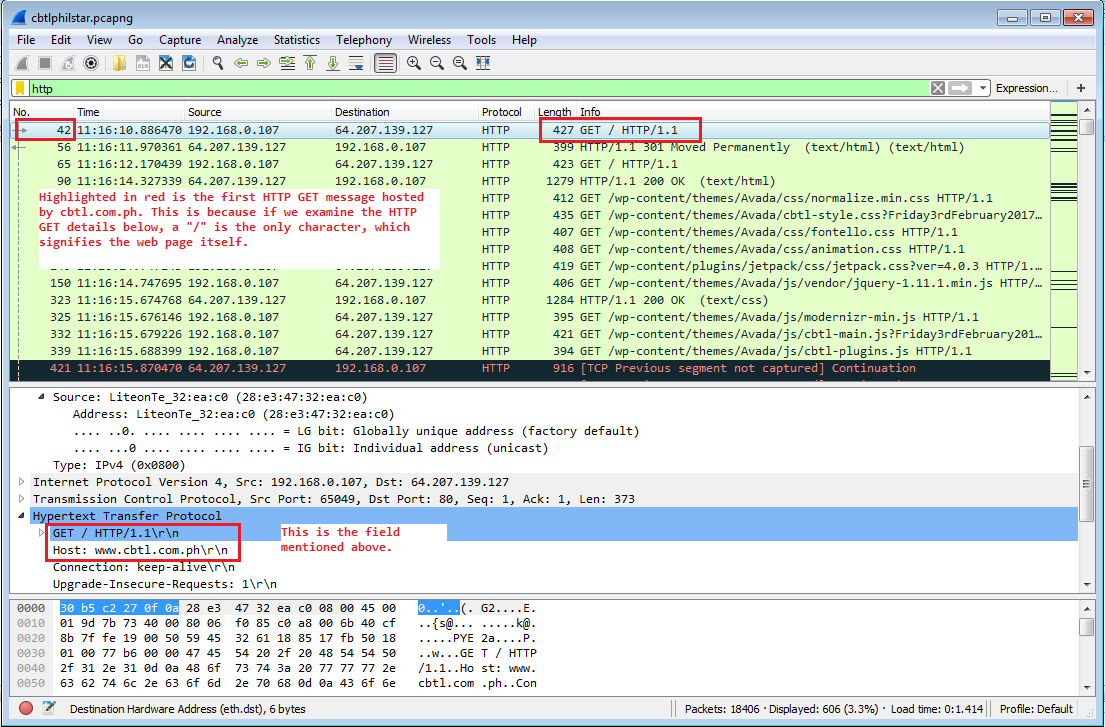
\includegraphics[scale=0.4]{Q1}
\end{center}

\item
Packet \#3066
\begin{center}
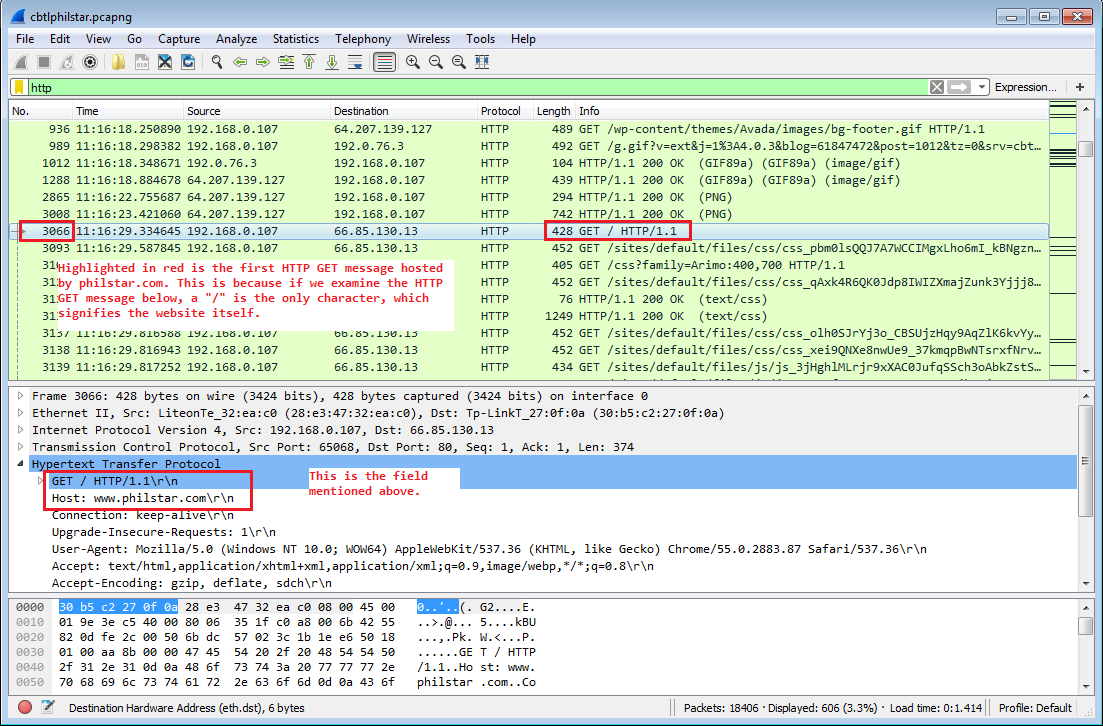
\includegraphics[scale=0.4]{Q2}
\end{center}

\item
\textbf{Source Address:} LiteonTe\_32:ea:c0 (28:e3:47:32:ea:c0) \\
\textbf{Destination Address:} Tp-LinkT\_27:0f:0a (30:b5:c2:27:0f:0a)
\begin{center}
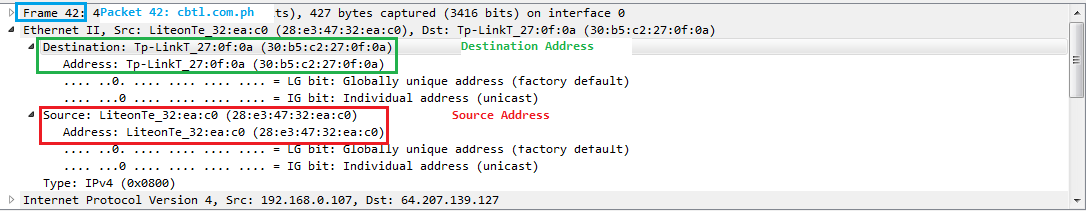
\includegraphics[scale=0.5]{Q3}
\end{center}

\item
\textbf{Source Address:} LiteonTe\_32:ea:c0 (28:e3:47:32:ea:c0) \\
\textbf{Destination Address:} Tp-LinkT\_27:0f:0a (30:b5:c2:27:0f:0a)
\begin{center}
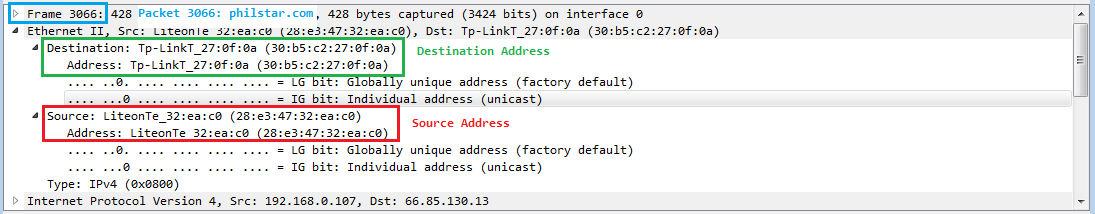
\includegraphics[scale=0.5]{Q4}
\end{center}

\item
The source address signifies the MAC Address of the terminal which allows it to conenct to a network.

\item
The destination address signifies the MAC Address of the DNS Server that allows the terminal to connect to the Internet. Since the two websites have the same MAC Address, they are hosted by the same server.

\item
The two addresses are the same which makes sense considering that the source is coming from the same computer terminal, having a single and unique MAC Address.

\item
The two addresses are the same. It makes sense because a single server hosts the two websites despite having two different IP Addresses.

\item
\textbf{ifconifg} stands for \textit{"interface configuration"} (equiv. \textbf{ipconfig}, \textit{"internet protocol configuration"}). It is used to view and change the configuration of the system's network interfaces. \footnote{http://www.computerhope.com/unix/uifconfi.htm}

If we consider the terminal's output for \textbf{ifconfig}, the values are not consistent with that of the values in the packet trace. This is because the trace was not generated in the same terminal as the one where \textbf{ifconfig} is performed.

\begin{center}
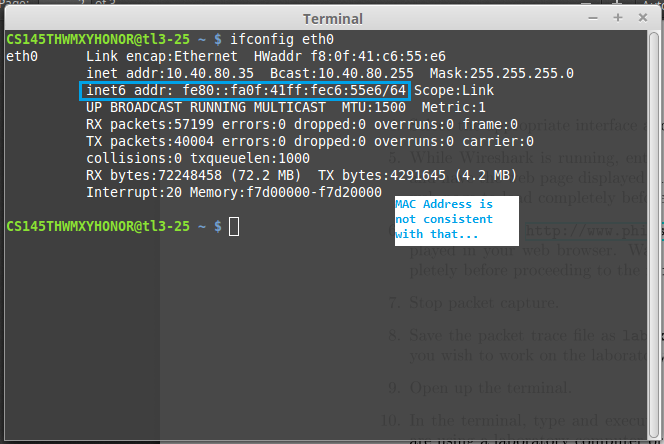
\includegraphics[scale=0.5]{terminal2}
\end{center}

\begin{center}
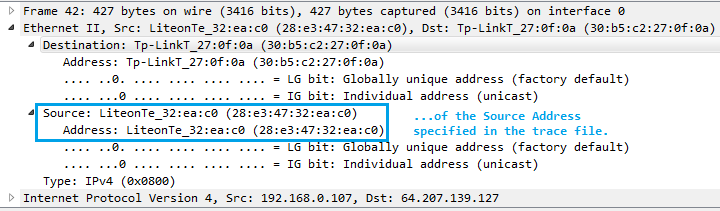
\includegraphics[scale=0.75]{9}
\end{center}

\end{enumerate}

\end{document}